\documentclass{uebblatt}

\newcommand{\cont}{\mathrm{cont}}
\newcommand{\http}{http:/\kern-.2em/\kern-0.03em}

\begin{document}

\maketitle{12}{\href{https://en.wikipedia.org/wiki/P-adic_number}{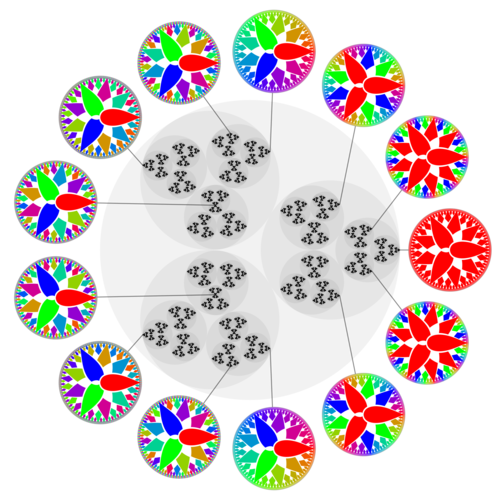
\includegraphics[scale=0.24]{images/p-adic-numbers}}}

\begin{aufgabe}{m+m+2+1+1}{Spiel und Spaß mit~$p$-adischen Zahlen}
Sei~$\ZZ_p$ der Ring der~$p$-adischen Ganzzahlen, konstruierbar
als~$\varprojlim_n \ZZ/(p^n)$ oder Vervollständigung von~$\ZZ$ bezüglich
der~$(p)$-adischen Topologie.
\begin{enumerate}
\item Sei~$f \in \ZZ[X]$ ein Polynom, das modulo~$p$ eine einfache Nullstelle
besitzt. Zeige, dass~$f$ in~$\ZZ_p$ eine Nullstelle besitzt.
\item Sei~$n$ eine zu~$p$ teilerfremde ganze Zahl. Zeige, dass~$n$ in~$\ZZ_p$
invertierbar ist.
\item Berechne $\lim_{n \to \infty} \frac{1}{1 + p^n}$ und $\lim_{n \to \infty}
\frac{p^n}{1 + p^n}$ in~$\RR$ und in~$\ZZ_p$.
\item Seien~$x$ und~$y$ ganze Zahlen. Finde eine Folge~$p$-adischer Zahlen, die
in~$\RR$ gegen~$x$ und in~$\ZZ_p$ gegen~$y$ konvergiert.
\item Gibt es in~$\ZZ_{13}$ eine Quadratwurzel aus~$-1$?
\end{enumerate}
\end{aufgabe}

\begin{aufgabe}{3+m+3+1}{Hensels Lemma}
Sei~$A$ ein Ring. Sei~$f \in A[X]$ ein
Polynom, das modulo einem Ideal~$\aaa$ eine einfache Nullstelle besitzt: ein Element~$x_1
\in A$ mit~$f(x_1) \equiv 0$ modulo~$\aaa$, sodass es ein Element~$y \in A$
mit~$f'(x_1) y \equiv 1$ modulo~$\aaa$ gibt.
Wir definieren für~$n \geq 1$: $x_{n+1} \defeq x_n - y f(x_n)$.
\begin{enumerate}
\item Zeige für alle~$n \geq 1$, dass $x_n \equiv x_m \pmod{\aaa^m}$ für
alle~$m < n$ und dass~$f(x_n) \equiv 0 \pmod{\aaa^n}$.
% Tipp: formale Taylorentwicklung
\item Zeige, dass~$(x_n)_n$ eine Cauchy-Folge bezüglich der~$\aaa$-adischen
Topologie ist.
\item Sei~$A$ vollständig bezüglich dieser Topologie. Zeige,
dass~$f$ eine Nullstelle in~$A$ besitzt.
\item Unter welchem Namen ist das Konstruktionsverfahren für die~$x_n$ bekannt?
Bewundere die Einheit der Mathematik.
\end{enumerate}
\end{aufgabe}

\begin{aufgabe}{2}{Regularität unter Vervollständigung}
Sei~$x$ ein reguläres Element in einem topologischen Ring~$A$. Zeige, dass das
Bild von~$x$ unter dem kanonischen Homomorphismus~$A \to \hat A$ ebenfalls regulär ist.
\end{aufgabe}

\begin{aufgabe}{m}{Potenzreihenentwicklung der Quadratwurzel}
Sei~$K$ ein Körper mit~$2 \neq 0$. Zeige: Es gibt eine Potenzreihe~$p \in
\ps{K}$ mit~$p^2 = 1 + X$.
\end{aufgabe}

\end{document}
